\subsection{Endogenous Transformations}
\label{sec:slco:endogenous}
For each of the semantic gaps and platform gaps described in Section~\ref{sec:slco:language-gaps}, we implemented an endogenous model transformation that bridges this gap.
To keep these transformations simple, they can only be applied to models adhering to certain conditions.
In addition to the transformations that bridge the gaps, we implemented transformations that refine models to ensure that they adhere to the aforementioned conditions.

\subsubsection{Synchronized Communication over Asynchronous Channels}
\label{subsubsec:slco:sync2async}
To bridge the semantic gap between languages offering synchronous communication and languages that do not, we implemented two transformations.
Both transformations take an \SLCO model and a synchronous channel as input, and produce a model in which this channel is replaced by an asynchronous, lossless channel and the objects that communicate over this channel are adapted such that they communicate asynchronously.

\begin{figure}[hbt]
  \centering
  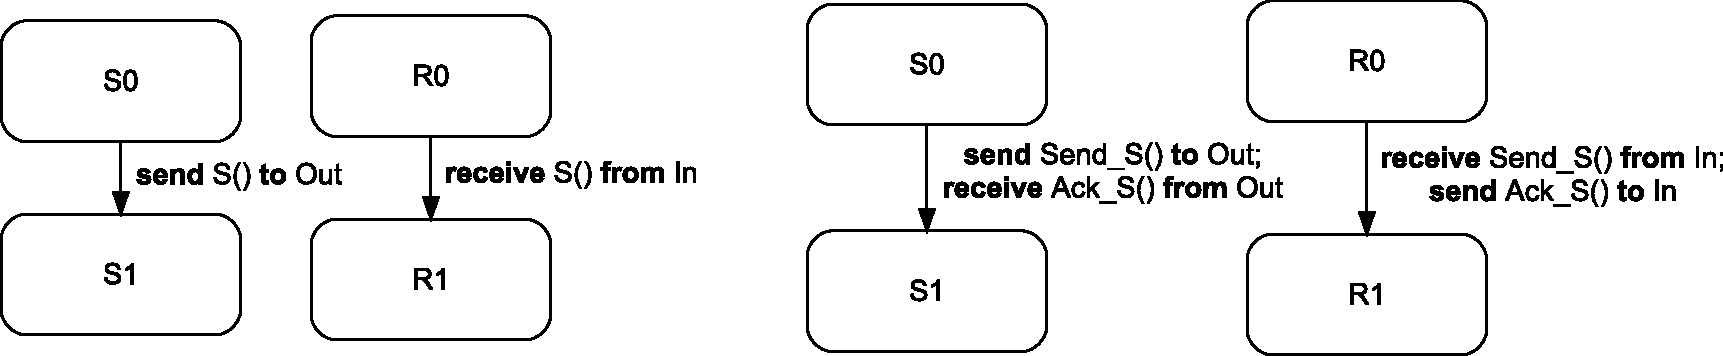
\includegraphics[scale=0.45]{slco/figs/transformations/s2a_simple}
  \caption{State machines before and after applying the simple version of \Transformation{as}}
  \label{fig:slco:trans:assimple}
\end{figure}

The first transformation is simple, but can only be applied to models that do not contain states with multiple outgoing transitions if one of these transitions starts with a statement that sends a signal over the synchronous channel.
The transformation ensures that the behavior of the model is still as desired by adding acknowledgment signals for synchronization.
Whenever a signal is sent, the receiving party sends an acknowledgement indicating that the signal has been received.
The sending party waits until it receives this acknowledgement.
In this way, synchronization is achieved.
On the left of Figure~\ref{fig:slco:trans:assimple}, two partial state machines are shown that send and receive a signal~\SLCOSignalName{S}.
Initially, ports~\SLCOPort{In} and~\SLCOPort{Out} are connected by a synchronous channel.
After transformation, acknowledgements are added, as shown on the right of the figure, and the synchronous channel is replaced with an asynchronous, lossless channel.
This transformation is described in more detail in Appendix~\ref{ap:transformations-slco}, and its correctness is discussed in Chapter~\ref{chap:reusable-correct-transformations} and Appendix~\ref{ap:proof}.

\begin{figure}[hbt]
  \centering
  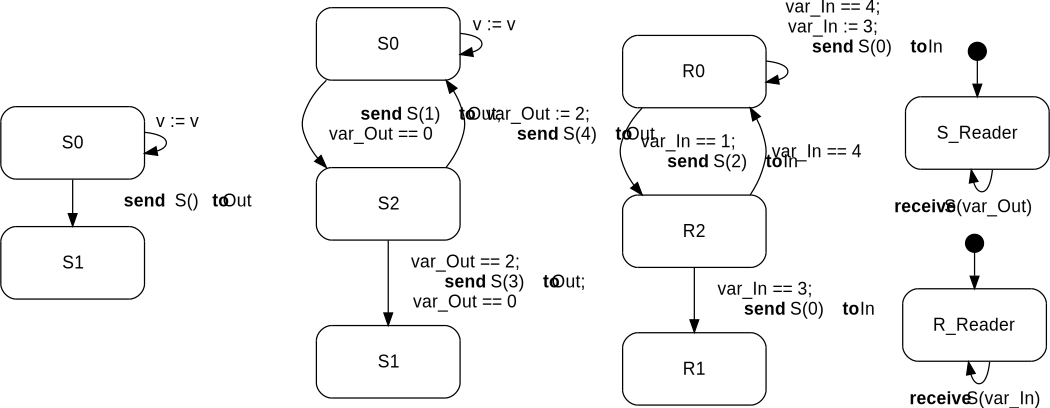
\includegraphics[scale=0.45]{slco/figs/transformations/s2a_complex}
  \caption{State machines before and after applying the general version of \Transformation{as}}
  \label{fig:slco:trans:ascomplex}
\end{figure}

The second transformation can be applied to any \SLCO model, but is more complex.
The partial state machine on the left of Figure~\ref{fig:slco:trans:ascomplex} shows an example of a situation where the transformation described above cannot be applied.
State~\SLCOState{S0} has multiple outgoing transitions, and one of these transitions starts with a statement that sends a signal.
In such situations, a more complex protocol has to be applied to ensure that the behavior of the model before and after transformation is the same, apart from the communication over the channel that is replaced.
Also in this example, ports~\SLCOPort{In} and~\SLCOPort{Out} are initially connected by a synchronous channel, which is replaced by an asynchronous, lossless channel.
In Figure~\ref{fig:slco:trans:ascomplex}, the second partial state machine from the left shows how the sending state machine is affected by the transformation, and the third partial state machine from the left shows how the receiving state machine is affected.
Additionally, two other state machines are added to the model, which are shown on the right of Figure~\ref{fig:slco:trans:ascomplex}.
State machine~\SLCOStateMachine{S\_Reader} is added to the object that sends signals, and state machine~\SLCOStateMachine{R\_Reader} is added to the object that receives signals.
Together with these state machines, the sender and receiver implement a protocol that ensures that states~\SLCOState{S1} and~\SLCOState{R1} are only reached if the communication between the sender and receiver was successful.
Furthermore, as long as the sender and receiver are unable to communicate, all enabled outgoing transitions of states~\SLCOState{S0} and~\SLCOState{R0} can be made.
Appendix~\ref{ap:transformations-slco} provides a more detailed description of this transformation.

The protocol that is employed by this transformation is not straightforward.
Therefore, we used the state-space generator for \SLCO described in Chapter~\ref{chap:prototype-semantics} for feedback during its development.
Informally, the protocol consists of the following steps.
Initially, the value of variable~\SLCOVariable{var\_Out} is equal to~0, and the value of variable~\SLCOVariable{var\_In} is equal to~3.
First, the sending object sends a signal~\SLCOSignal{S}{1} to indicate that it wants to communicate.
It can proceed to state~\SLCOState{S2} if all previous signals have been acknowledged by the receiving object, which is the case if variable~\SLCOVariable{var\_Out} is equal to~0.
The signal sent by the sending object is received by state machine~\SLCOStateMachine{R\_Reader}, and the value of its argument is stored in~\SLCOVariable{var\_In}.
Once the receiving object is informed of the intent of the sending object by means of the execution of statement~$\SLCOVariable{var\_In}==1$, it sends a signal~\SLCOSignal{S}{2} to indicate that it is ready to communicate.
Once this signal has been received and the value of its argument has been stored in variable~\SLCOVariable{var\_Out} by state machine~\SLCOStateMachine{S\_Reader}, the sending object may choose to complete the communication by sending signal~\SLCOSignal{S}{3}.
Alternatively, it may choose to cancel the communication by sending signal~\SLCOSignal{S}{4}.
Upon receiving one of these signals, the receiving object can take the transition to state~\SLCOState{R1} if the communication has been completed successfully, or take the transition to state~\SLCOState{R0} if it has been canceled.
Either way, it acknowledges the reception of the signal of the sending object by sending a signal~\SLCOSignal{S}{0}.
The state machines~\SLCOStateMachine{S\_Reader} and~\SLCOStateMachine{R\_Reader} ensure that the statements that send signals cannot be blocked, by emptying the buffers associated to the channels continuously.
It is possible that the sending object sends signal~\SLCOSignal{S}{4} after sending signal~\SLCOSignal{S}{1}, while the receiving object remains in state~\SLCOState{R0}.
The self-loop on state~\SLCOState{R0} ensures that an acknowledgement is also sent in this situation.

In the remainder, the simple version of this transformation is referred to as~\TSim, and the general version is referred to as~\TGen.
In cases where it is not relevant which of these two transformations is applied, the abbreviation~\Transformation{as} is used.

\subsubsection{Lossless Communication over a Lossy Channel}
\label{subsubsec:slco:ll}

Transformation~\Transformation{ll} implements lossless communication over a lossy channel by introducing auxiliary objects that implement a concurrent version of the Alternating Bit Protocol~(ABP)~\cite{Bartlett1969} known as the Concurrent Alternating Bit Protocol (CABP)~\cite{Baeten2002}.
This transformation is only applicable to unidirectional channels that are used to communicate signals named \SLCOSignalName{Signal} and whose only argument is a string.

\begin{figure}[hbt]
  \centering
  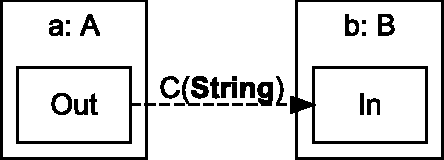
\includegraphics[scale=0.45]{slco/figs/transformations/Communication_Lossless2Lossy}
  \caption{Two objects communicating over an asynchronous, lossless channel}
  \label{fig:slco:ll-comm-before}
\end{figure}

Figure~\ref{fig:slco:ll-comm-before} shows a model consisting of two objects~(\SLCOObject{a} and~\SLCOObject{b}) that communicate over an asynchronous, lossless channel~(\SLCOChannel{C}).
After transformation, channel~\SLCOChannel{C} is replaced by the channels~\SLCOChannel{c1} to~\SLCOChannel{c6} and four objects that implement the CABP, as shown in Figure~\ref{fig:slco:ll-comm-after}.
Object~\SLCOObject{a} is connected to an object named~\SLCOObject{sender}, which communicates over an asynchronous, lossy channel~\SLCOChannel{c2} with an object named~\SLCOObject{receiver}.
The object named~\SLCOObject{receiver} is in turn connected to the object~\SLCOObject{b}.
After transformation, objects~\SLCOObject{a} and~\SLCOObject{b} communicate with each other via the aforementioned objects, instead of directly.
Objects~\SLCOObject{a} and~\SLCOObject{b} are connected to these objects by synchronous channels.
After receiving a signal from object~\SLCOObject{a}, object~\SLCOObject{sender} repeatedly sends this signal over channel~\SLCOChannel{c2} until it receives an acknowledgement from object~\SLCOObject{ar}, to which it is connected via the synchronous channel~\SLCOChannel{c6}.
After receiving a signal over channel~\SLCOChannel{c2}, object~\SLCOObject{receiver} forwards this signal to object~\SLCOObject{b} and instructs object~\SLCOObject{as} to continuously acknowledge the reception of this signal.
Object~\SLCOObject{as} does this by continuously sending signals over the asynchronous, lossy channel~\SLCOChannel{c5}.
The acknowledgement sent by object~\SLCOObject{as} contains a two-valued argument that is used by object~\SLCOObject{ar} to assess whether a particular acknowledgement signal was already received before.
Once object~\SLCOObject{ar} has received a new acknowledgement, it notifies object~\SLCOObject{sender}.
After receiving such a notification, object~\SLCOObject{sender} is able to receive a new signal from object~\SLCOObject{a} and transmit this signal over channel~\SLCOChannel{c2}.

In Figure~\ref{fig:slco:cabp}, the four state machines are shown that specify the behavior of the four objects that implement the CABP.
To show which state machine is part of which class, the names of the states have been chosen such that they reflect the names of the classes and objects.

\begin{figure}[hbt]
  \centering
  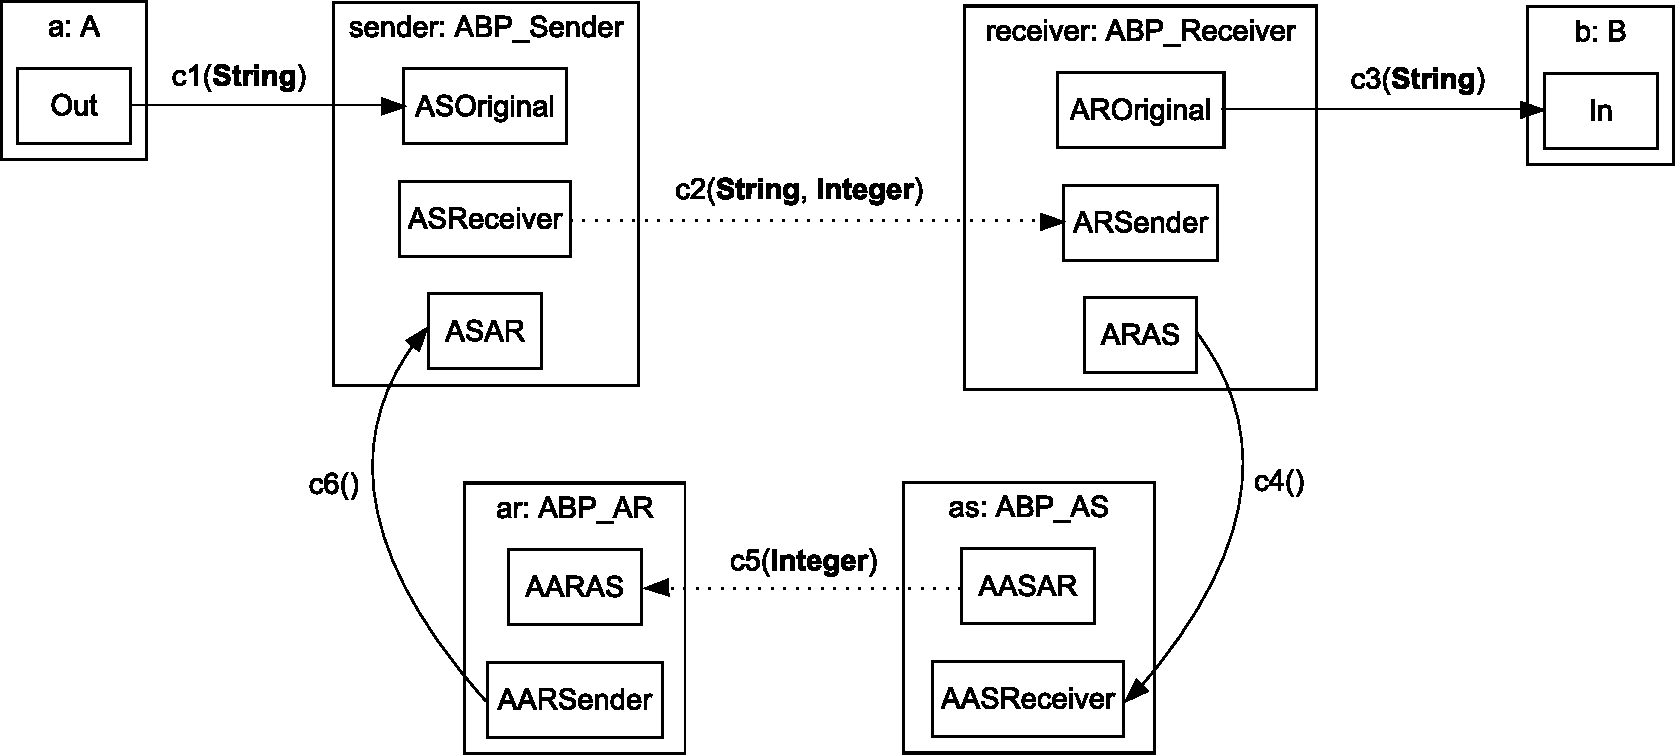
\includegraphics[scale=0.45]{slco/figs/transformations/Communication_Lossless2Lossy_ll}
  \caption{Two objects that communicate via the CABP}
  \label{fig:slco:ll-comm-after}
\end{figure}



\begin{figure}[hbt]
  \centering
  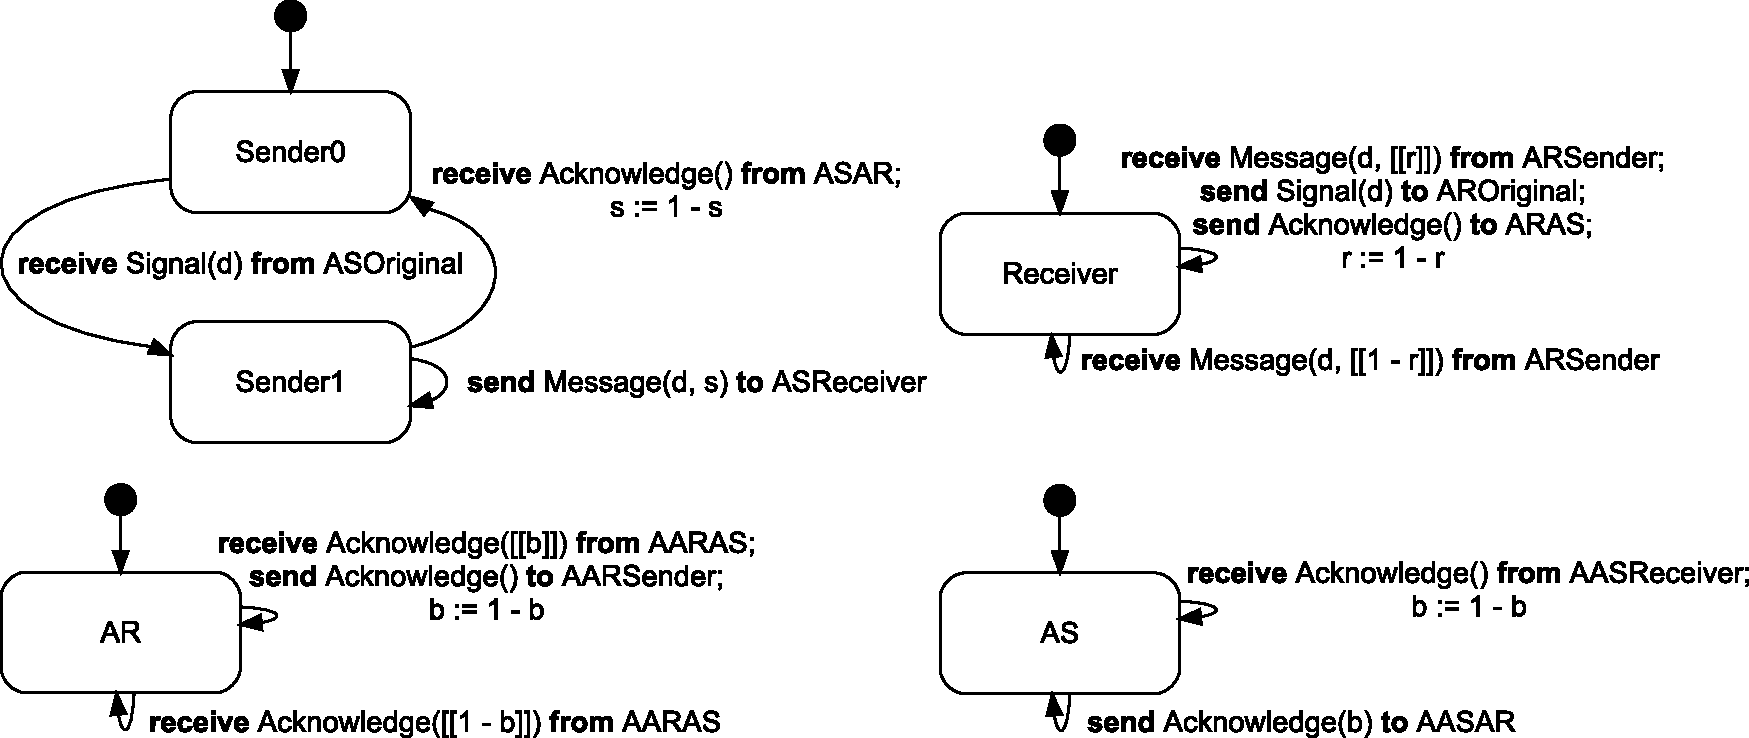
\includegraphics[scale=0.45]{slco/figs/transformations/ABP}
  \caption{Four state machines implementing the CABP}
  \label{fig:slco:cabp}
\end{figure}

\subsubsection{Adding Delays to Transitions}
Transformation~\Transformation{time} takes a model and a set of transitions as input, and adds delay statements to these transitions.
This transformations is used to control the frequency of the acknowledgments sent by the objects implementing the CABP.
Because it reduces the number of signals that are sent, it also reduces the number of collisions between messages sent via infrared on the Lego Mindstorms platform.

%%%

\subsubsection{Replacing Strings by Integers}
Transformation~\Transformation{int} replaces each string constant in an \SLCO model with a unique integer constant and changes the type of all string variables and arguments to integer.
This transformation deals with the fact that \NQC does not offer strings.

\subsubsection{Making the Sender of a Signal Explicit}
When multiple objects broadcast signals with the same name and number of arguments over the same medium, the receiving object cannot determine the origin of such a signal.
This situation arises when multiple \RCX controllers communicate with each other, because they communicate by broadcasting messages via infrared.
To enable a receiving controller to determine the origin of each signal it receives, transformation~\Transformation{ic} can be applied to a model.
This transformation takes a model and a set of channels as input, and adds an index to all signal names that identifies the channel over which these signals are sent.

\subsubsection{Reducing the Number of Objects}
\label{subsubsec:slco:merge}
Transformation~\Transformation{merge} merges multiple objects into one object.
Given a model and a set of objects, it creates a new object that contains all the variables, ports, and state machines contained by the objects provided as input.
By reducing the number of objects in a model, it bridges the corresponding gap between \SLCO and \NQC.
If any of the objects that are being merged communicate over synchronous channels, then this form of communication is replaced by communication using shared variables.
Transformation~\Transformation{merge} is only applicable to objects that satisfy the following condition: each pair of state machines that are part of two communicating objects must communicate over a unique unidirectional, synchronous channel.

\begin{figure}[hbt]
  \centering
  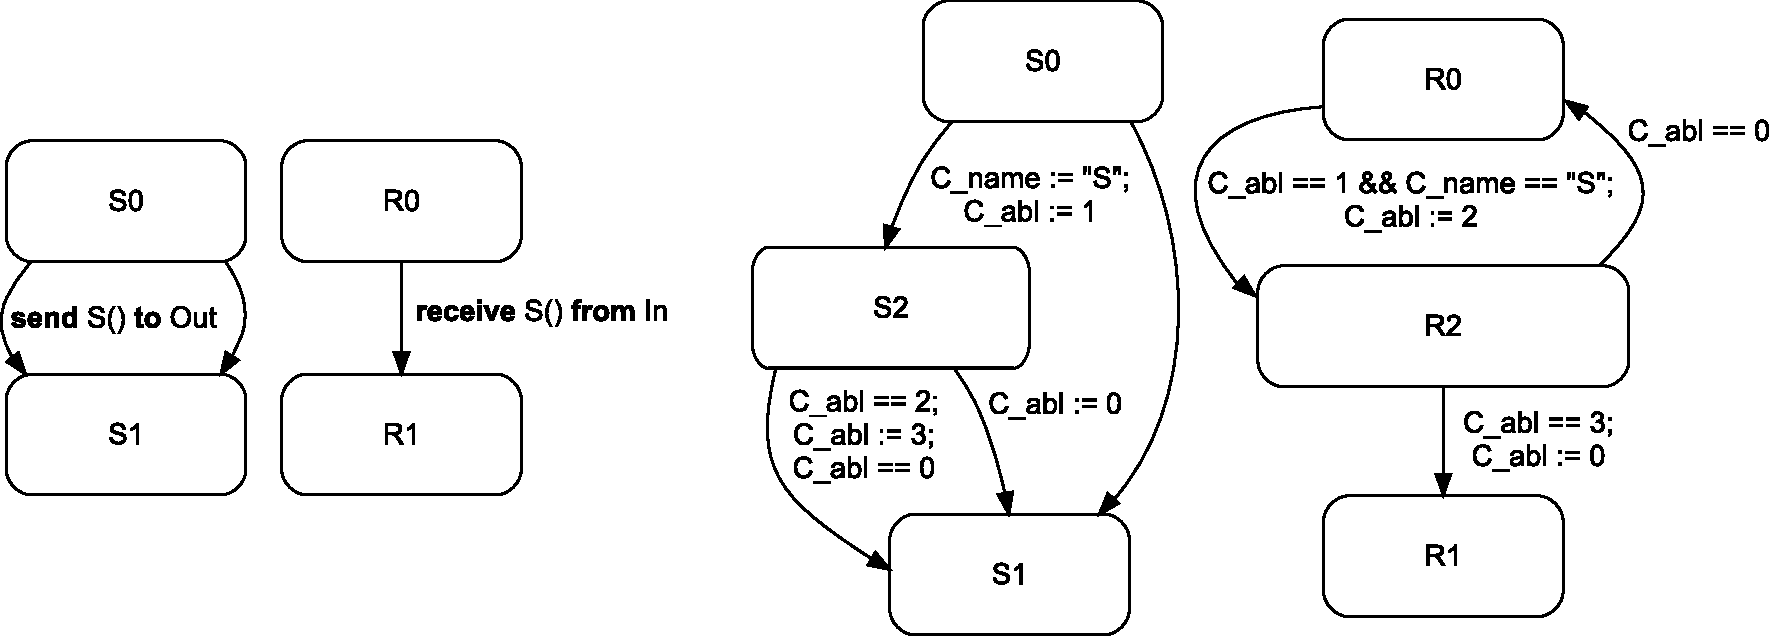
\includegraphics[scale=0.45]{slco/figs/transformations/MergeObjects}
  \caption{Two state machines before and after merging objects}
  \label{fig:slco:merge}
\end{figure}

Figure~\ref{fig:slco:merge} shows how communication over a synchronous channel is replaced by communication using shared variables.
The two partial state machines on the left of the figure are part of two separate objects and communicate with each other by sending and receiving signals over a synchronous channel that connects ports~\SLCOPort{In} and~\SLCOPort{Out}.
After merging these two objects, the state machines are adapted as shown on the right of the figure and communicate using the shared variables~\SLCOVariable{C\_name} and~\SLCOVariable{C\_abl}.
Variable~\SLCOVariable{C\_name} is used to store and retrieve the names of the signals that are being exchanged, and variable~\SLCOVariable{C\_abl} encodes the states of the employed communication protocol.
The sending state machine sets the value of~\SLCOVariable{C\_abl} to~1 to indicate that it wants to communicate.
The receiving state machine indicates that it is also able to communicate by setting the value of~\SLCOVariable{C\_abl} to~2.
If both state machines are able to communicate, the sending state machine can complete the communication process by setting~\SLCOVariable{C\_abl} to 3.
It may also choose to cancel the communication by setting~\SLCOVariable{C\_abl} to~0.
The receiving state machine acknowledges successful completion of the communication process by setting~\SLCOVariable{C\_abl} to~0.

\subsubsection{Making all Signal Names Equal}
\label{subsubsec:slco:endogenous:arg}
To keep the transformation that adds the CABP as simple as possible, our implementation of the CABP takes signals with a fixed name as input, transfers them over a lossy channel, and delivers them at the receiving end.
Before this instance of the CABP can be used to substitute an asynchronous, lossless, unidirectional channel, the signal names that are sent over this channel have to be changed into this fixed name.
Transformation~\Transformation{arg} adapts signals such that their name is changed into this fixed name and the name of the original signal is sent as an argument of the resulting signal.
For example, the statement~\SLCOSendSignal{Block}{}{O} is replaced by the statement~\SLCOSendSignal{Signal}{``\it{Block}"}{O}.

\subsubsection{Replacing a Bidirectional Channel by two Unidirectional Channels}
Our implementation of the CABP can only substitute asynchronous, lossless, unidirectional channels.
In some cases, therefore, a transformation is needed that replaces communication over a bidirectional channel by communication over two unidirectional channels before transformation~\Transformation{ll} can be applied.
Transformation~\Transformation{uni} performs this task.

\subsubsection{Exclusive Channels for Pairs of State Machines}
\label{subsubsec:slco:endogenous:ex}
Transformation~\Transformation{merge} cannot merge objects if multiple state machines that are part of an object communicate via the same port.
To modify models that do not adhere to this condition, we implemented a transformation~\Transformation{ex} that replaces a channel between a pair of objects with a number of identical channels.
For each pair of communicating state machines that are part of the two objects, a channel is introduced.

\begin{figure}[hbt]
  \centering
  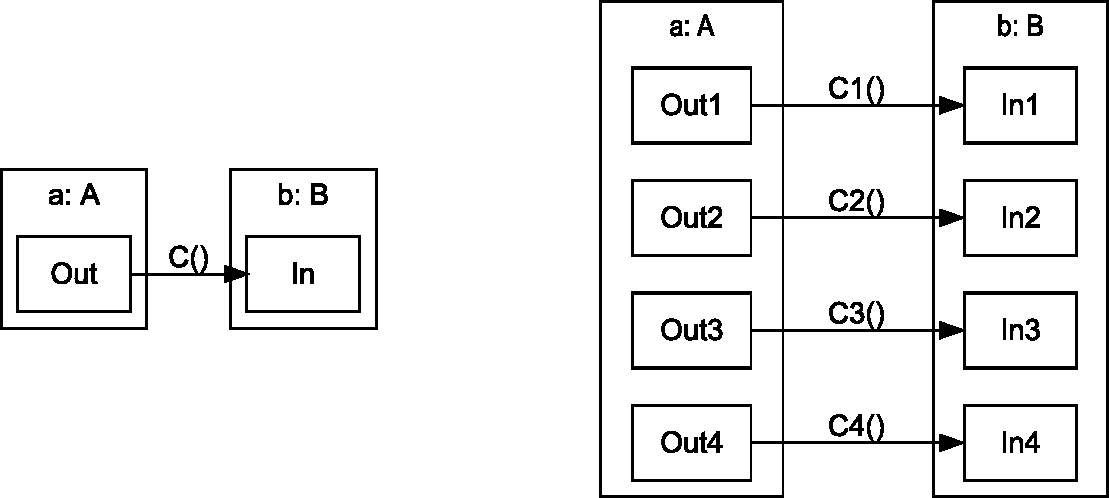
\includegraphics[scale=0.45]{slco/figs/transformations/ExclusiveChannels_Communication}
  \caption{Communication before and after adding exclusive channels}
  \label{fig:slco:excomm}
\end{figure}

On the left of Figure~\ref{fig:slco:excomm}, two objects are shown that communicate over a single channel.
Both objects contain two state machines (which are not shown in this type of diagram) that communicate over this channel.
After applying transformation~\Transformation{ex}, the channel is replaced by four channels, as shown on the right of Figure~\ref{fig:slco:excomm}.

\begin{figure}[hbt]
  \centering
  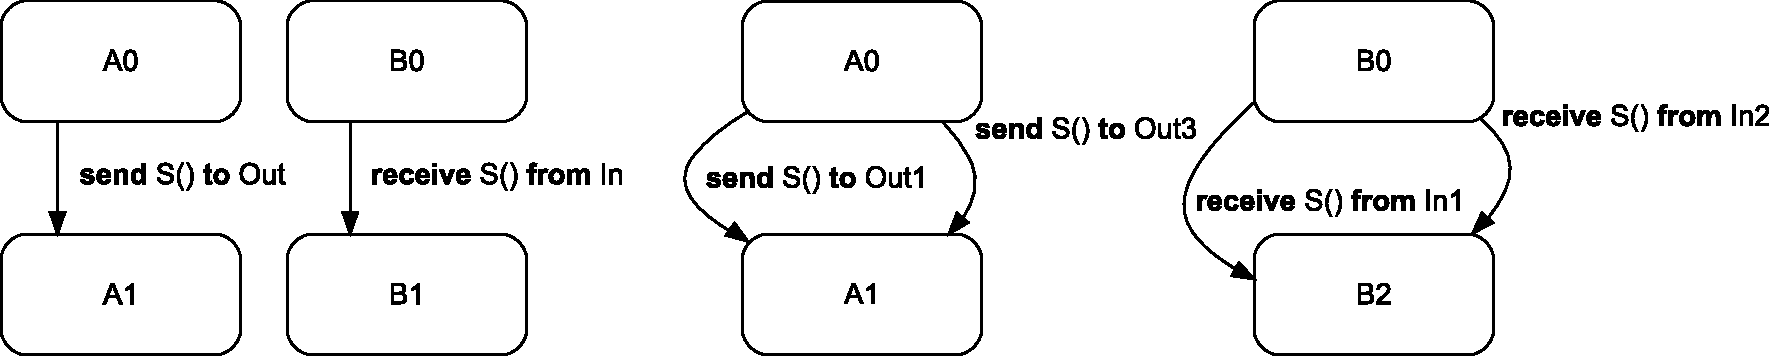
\includegraphics[scale=0.45]{slco/figs/transformations/ExclusiveChannels_Behavior}
  \caption{State machines before and after adding exclusive channels}
  \label{fig:slco:exsm}
\end{figure}

As a part of the process of replacing a channel by multiple channels, transformation~\Transformation{ex} modifies the state machines that communicate over these channels.
Before transformation, both state machines that are part of object~\SLCOObject{a} send signals via port~\SLCOPort{Out}, and both state machines that are part of object~\SLCOObject{b} receive signals via port~\SLCOPort{In}.
After transformation, one of the state machine of object~\SLCOObject{a} sends signals via ports~\SLCOPort{Out1} and~\SLCOPort{Out3}, and the other uses ports~\SLCOPort{Out2} and~\SLCOPort{Out4}.
The receiving state machines are modified in a similar fashion.
Figure~\ref{fig:slco:exsm} shows parts of one of the state machine of object~\SLCOObject{a} and parts of one of the state machines of object~\SLCOObject{b} before and after transformation.
The names of the states of these partial state machines correspond to the names of the classes they belong to.
The situation before transformation is illustrated on the left of the figure, and the situation after transformation is shown on the right.
%Before transformation, as shown on the left of the figure, state~\SLCOState{A0} has only one outgoing transition.
%When making this transition from state~\SLCOState{A0} to state~\SLCOState{A1}, a signal is sent via port~\SLCOPort{Out}.
%State~\SLCOState{B0} also has only one outgoing transition before transformation.
%When a signal is received via port~\SLCOPort{In}, the transition to state~\SLCOState{B1} is made.


\subsubsection{Reducing the Number of Channels}
When two objects are connected by more than one channel, these channels can be merged into one if they have the same type and directionality, and support the same argument types.
Therefore, we implemented a transformation~\Transformation{mc} that merges multiple channels between a pair of objects into one channel.
Merging channels is a way of optimizing models because it can be used to reduce the number of instances of the CABP that need to be added.

\subsubsection{Cloning Classes}
Many of the transformations described above use two auxiliary transformations.
One of these transformations takes a model and a channel as input, and clones the classes of the objects that communicate over this channel.
After applying this transformation, the objects that communicate over the channel are instances of the new cloned classes, and all remaining instances of the original classes remain unchanged.
This transformation ensures that all transformations that alter objects that communicate over a certain channel only affect these particular objects.

\begin{figure}[hbt]
  \centering
  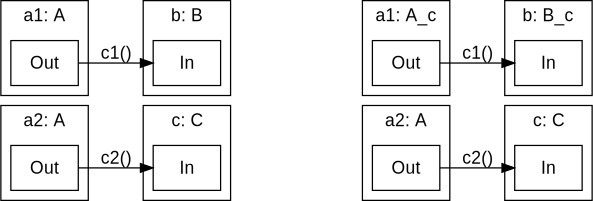
\includegraphics[scale=0.45]{slco/figs/transformations/CloneClasses}
  \caption{A model before and after cloning classes}
  \label{fig:slco:clone}
\end{figure}

Figure~\ref{fig:slco:clone} shows the communication diagram of a model before and after applying this transformation.
After transformation, the classes of the objects communicating over channel~\SLCOChannel{c1} are cloned.
In the resulting model, object~\SLCOObject{a1} is an instance of class~\SLCOClass{A\_c} and object~\SLCOObject{b} an instance of class~\SLCOClass{B\_c}.

\subsubsection{Removing Unused Classes}
The second auxiliary transformation used by the transformations described above removes all uninstantiated classes from a model.
The model depicted on the right of Figure~\ref{fig:slco:clone}, for example, no longer contains an instance of class~\SLCOClass{B}, which means that this class can be removed without affecting the system specified by the model.

%These two transformations are not shown in Figure~\ref{fig:TransformationSequences} to increase its readability.

%%%%%%%%%%%%%%%%%%%%%%%%%%%%%%%%%%%%%%%%%%%%%%%%%%%%
%%%%%%%%%%%%%%%%%%%%%%%%%%%%%%%%%%%%%%%%%%%%%%%%%%%%
%%%%%%%%%%%%%%%%%%%%%%%%%%%%%%%%%%%%%%%%%%%%%%%%%%%%
%%%%%%%%%%%%%%%%%%%%%%%%%%%%%%%%%%%%%%%%%%%%%%%%%%%%


